\chapter{Background Study}

\section{Quick Response Codes}

Quick Response Codes (QR Codes) are two dimensional bar codes that were initially
 used in Japanese car factories to allow computers to track the progress of
 an item on a production line [\cite{website:denso-qrcode}]. The technology has
 since evolved and matured and is today widely used in the media industry for storing some
 data, such as a web address or phone number. See Figure \ref{qrcode} for an example of a QR
 code.
 
\begin{figure}[h]
\centering
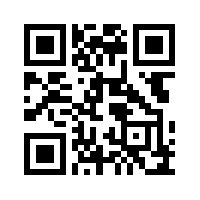
\includegraphics[scale = 0.7]{qrcode_voorbeeld.png}
\caption{Example of simple QR Code.}
\label{qrcode}
\end{figure}
 
 QR Codes can store up to 2,953 [\cite{website:denso-qrcode}] bytes of
 data, which is accessible by scanning the code, with either a laser or a
 digital camera. To scan a QR Code requires a camera that can produce a
 digital image of appropriate quality. This image is then processed by a QR Code library, e.g. the
 well-known ZXing library (see section \ref{sec:zbar}), which decodes the picture and outputs
 the data inside the code. Cellphones are commonly used today because of its portability,
 increasingly powerful hardware and the QR Code technology's simplicity.
 However, an image with a QR Code in can be decoded by any computer with the relevant hardware
 and libraries installed.

\subsection{Zebra Crossing Library}
\label{sec:zbar}

The Zebra Crossing Library (ZXing for short) is a well-known QR Code coding and decoding
library.
It is commonly built into smart phone applications to decode a static image or a video stream,
but a desktop version of the library, called ZBar, is also available and works in a similar
manner. 

To date there has been at least 50 million downloads of the ZXing
bar code scanner app on the Android platform alone, and it currently lies $98^{th}$ in the top
100 of the Google Play Store's most downloaded list [\cite{website:barcodescanner}].

\section{Near Field Communication}

Near Field Communication (NFC) is a relatively new communication standard in the world of
wireless technology. It allows two NFC-enabled devices to wirelessly transmit data by bringing
them to close to one another, typically around 4 centimeters.

This technology is commonly found in modern cellphones. However, recently the technology has
been ported to other platforms such as a desktop computer and Arduino. This adds a new
dimension to wireless inter-device communication and makes projects such as this more
feasible.

\subsection{libnfc}

Libnfc is a open-source library for Linux systems [\cite{website:libnfc}]. It allows a
desktop computer to communicate with a NFC device based on the PN53 series of NFC chips
[\cite{website:libnfc-hardware}]. Recent versions have made provision for the use of a PN532
breakout board that can be used by a Raspberry Pi. 

It is currently in version 1.7 and is classified as a `mature' library. 

\subsubsection{nfcpy}

Nfcpy is a Python interface for the libnfc library and it allows for peer-to-peer communication
between a cellphone and desktop-based NFC controller using the NFC Data Exchange Format
(NDEF), the Simple NDEF Exchange Protocol (SNEP) and the Logical Link Control Protocol (LLCP).
These standards and protocols have been set by the NFC standard governing body, the NFC Forum
[\cite{website:nfc-forum}], to simplify and standardise data exchange between different
platforms and to make the user experience more pleasant.

Nfcpy is an open-source program, written and maintained by Stephen Tiedemann
[\cite{website:nfcpy}].

\subsection{Android}

Google's Android operating system is currently the most widely used cellphone operating system
being used word wide with, an estimated 80\% market share [\cite{website:android-marketshare}].
Other platforms, such as the Blackberry OS and Windows Phone, have also added NFC to their
latest phones, but they do not have the market penetration that Android currently has. 

It is also the platform which most aggressively promotes the use of NFC as an alternative 
payment option in modern retail outlets with applications such as Google Wallet
[\cite{website:android-wallet}].

\subsection{Radio Field Identification and Stellenbosch
University Student Cards}

NFC and Radio Frequency Identification (RFID) work in a similar manner: when two
devices  (e.g. cellphone, RFID tag, MiFare card, etc.), equipped with an antenna tuned to a
frequency  of 13.56MHz, come into close proximity, they transmit some form of data to one another.

However, there are some important difference between the two technologies. For example, a NFC
system is  an active system, meaning that the device's antenna is always powered and runs off
its own  power supply. NFC devices also have peer-to-peer (p2p) capabilities, meaning that the
two  devices can communicate with one another by both sending and receiving data.
RFID systems on the  other hand, work by having one device act as a listener and the other as a
sender [\cite{website:diff-nfc-rfid}] (e.g. the current SU's student entry control system).

\section{Web Server}

\subsection{Django Web Framework}

Django is a Python web server framework which focuses on easy setup and simple design. Here are
some of its features:

\begin{itemize}
  \item Fully handle HTTP GET and POST requests.
  \item Integration with SQL databases, e.g. MySQL, SQLite3, etc.
  \item HTML template design feature.
  \item Makes provision for the execution of Python scripts.
  \item It is fully scalable to commercial level servers.
\end{itemize}

This framework is expandable to commercial size servers that is accessible across the globe,
for example large websites such as Instagram and Pinterest are based on the Django framework
[\cite{website:django-sites}].

Django was initially developed by web programmers Adrian Holovaty and Simon Willison, from the
newspaper Lawrence Journal World [\cite{website:django-exist}]. It was first released in 2005
under the Berkeley Software Distribution (BSD) license and is completely free to use.

\subsection{Elastic Compute Cloud}

Elastic Cloud Compute (EC2) is a cloud computing service offered by Amazon Web Services (AWS).
It allows a user to rent a virtual computer from AWS from which to run their own applications.
These applications are most commonly web-based, in other words the virtual machines run a
web server that is accessible by anyone around the world.  

\subsection{Apache}

Apache is a popular web server application available on most platforms. For simplicity, the
details of Apache will not be discussed. However, a very notable feature of Apache is that it
is designed to be compatible and fully scalable with various web frameworks, such as Python's
Django, PHP's cgiapp and even C++'s Poco.

Apache is the currently the most popular web server application in use today, with an estimated
53.4\% of the world's servers running on apache [\cite{website:apache-usage}].

It was initially released by Robert McCool in 1995 under the Apache Licence, which makes it
free to use in any way. It is currently being maintained by the Apache Software Foundation. 

\section{Encryption}

Encryption is the act of encoding some data into seemingly unreadable garbage. This is done so
that unwanted parties cannot decode the data, but authorised parties can. This is most commonly
done with an encryption key and algorithm which specifies how the data was encoded and how it
can be decoded.

Encryption is most commonly used where sensitive information is being transmitted, e.g. banking
codes, personal e-mails, etc.

There are two main encryption schemes, namely symmetric and asymmetric encryption. 

\subsection{Symmetric Encryption}

In symmetric encryption, both parties, i.e. the sender and receiver, have to agree to a common
encryption key prior to the data transmission. In other words, the sender and receiver use the
same key to encrypt and decrypt the data. A famous example of symmetric encryption is the
Enigma cipher machine used by Nazi Germany in the Second World War. 

Unfortunately, due to the increase in knowledge around this type of encryption, various code
cracking methods have been developed since 1945, such as known and chosen plain-text attacks
[\cite{website:cipher-attacks}].

\subsection{Asymmetric Encryption}

More recently, asymmetric encryption, also known as public-key encryption, has come to the fore
as the new standard for encryption. It involves the use of a public and private key pair that
can be used to securely encrypt and sign a data package on the sender's side and to decrypt
and verify the data on the receiver's side.

This private and public key pair are mathematically related to one another according to the
algorithm in use (e.g. Elgamal or RSA, see sections \ref{sec:elgamal} and \ref{sec:rsa}). The
public key half of the pair is (in theory) publicly distributed to anyone who wants one (in
practise this is done differently to increase security). The great advantage of asymmetric
encryption is that even if the public half of the key is available, it is still very difficult,
and sometimes impossible, to get the private half of the key.

The encryption is most easily explained with a postal analogy:

Imagine two people, Alice and Bob, want to send each other secret messages through the public
mail. In other words, Alice wants to send Bob a secret message and she expects a secret reply
from Bob, and vice versa. 

In an asymmetric scheme, Bob can lock his letter to Alice with a padlock to which only she has
a key (she keeps this on her person at all times and does not show it to anyone, this
includes Bob). This open padlock represents the public key half of Alice's key. This
means that anyone can send Alice a secure message with a public key, which is easy to
get from Alice, and only Alice can ever unlock the message with her private key half of the
key pair. Similarly, Alice can lock her letter with a padlock which only Bob can ever open.

The great advantage that this has over symmetric encryption is that the decryption keys never
have to be exchanged between parties. This neutralises the risk of a middle-man attack,
analogous to a nosy postal worker called Eve who likes to read other peoples mail, that
intercepts the message and steals the key.
Also, if for example Bob has been careless and allowed Eve to see his key, his messages to
Alice will be compromised. However, the messages from anyone (including Bob) to Alice will
remain as secure as it was before Bob lost his key.

The data source can also be verified by using this key scheme. Referring once again to the
postal analogy:

To show Alice that it was indeed Bob who sent her the message, and not Eve for example, he can
send an extra message along with the original message. This extra message is locked with Bob's
key that he shares with no one (i.e. his private key). However, Bob has sent out special keys
to everyone who wants one. These special keys can \emph{only} be used to unlock the messages locked with Bob's
own private key. Therefore, if Alice, who received one of Bob's keys, can unlock this extra
message with that key, she knows that as long as Bob hasn't given anyone his private key, it
can only be his message. The reverse is also true if Alice wants to prove to Bob that it was
indeed here who sent him a message. 

\subsubsection{ElGamal}
\label{sec:elgamal}

The ElGamal encryption algorithm is an alternative to the more widely used  Ron Rivest, Adi
Shamir and Leonard Adleman (RSA) asymmetric encryption algorithm. ElGamal's security stems
from the `difficulty of computing discrete logarithms is a large prime modulus'.
[\cite{website:elgamal}]

The main advantage that the ElGamal algorithm has over RSA is that, firstly, a smaller key can
be used for a data string of the same length and secondly, due to the mathematics behind the
algorithm, it is almost certain that a different ciphertext will be generated each time a
string is encrypted.

However, a fairly large drawback of this algorithm is that the key needs to be at least twice
as long as the plain-text string that is being encrypted
[\cite{website:taher-elgamal}].

The algorithm was developed by Taher ElGamal in 1984 and is free to use under the GNU license.

\subsubsection{RSA}
\label{sec:rsa}

The Ron Rivest, Adi Shamir and Leonard Adleman (RSA) asymmetric encryption algorithm is a
widely used encryption standard. Its security is based on `the difficulty of factoring large 
integers' [\cite{website:elgamal}]. 

The main advantage of the RSA algorithm is its encryption and decryption speed. Also, the
encryptor has some measure of control over how long the produced ciphertext is going to be,
because the ciphertext will be as long as the encryption key used, provided the key is long
enough.

The RSA algorithm was developed by Ron Rivest, Adi Shamir and Leonard Adleman in 1978 and has
been widely used since 1993. 

\subsection{PyCrypto}

PyCrypto is a Python cryptography toolkit which contains various encryption algorithms and
key schemes, such as ElGamal, MD5 and RSA. It is currently registered under the public domain
and is free to use by anyone. It is maintained by the PyCrypto Team [\cite{website:pycrypto}].

\subsection{Base 64}

Base 64 is an encoding scheme which takes binary data and encodes it to ASCII characters. This
is most often used where the output of encrypted text is unreadable binary data and ASCII
characters are preferred because they are easier to read and transmit. 

It is also important to note that the the output of the base 64 encoding is approximately
33\% longer than the input string.

Here is an example of a base 64 encoded string:\\\\
\textbf{Original text:}\\
Hi, I'm a base 64 encoded string!\\
\textbf{Base 64 encoded output:}\\
SGksIEknbSBhIGJhc2UgNjQgZW5jb2RlZCBzdHJpbmch
